\section{PC总线类型} 

\subsection{PCI}
外设互联标准(或称个人电脑接口,Personal Computer Interface),实际应用中简称为PCI(Peripheral Component Interconnect),是一种连接电子计算机主板和外部设备的总线标准。一般PCI设备可分为以下两种形式:
直接布放在主板上的集成电路,在 PCI 规范中称作“平面设备”(planar device);或者
安装在插槽上的扩展卡。
PCI bus常见于现代的个人计算机中,并已取代了ISA和VESA 局部总线,成为了标准扩展总线。PCI 总线亦常见于其他电子计算机类型中。PCI总线最终将被PCI Express和其他更先进的技术取代,这些技术现在已经被用于最新款的电子计算机中。
PCI 规范规定了该总线的物理尺寸(包括线宽)、电气特性、总线时序和协议。该规范可从美国PCI-SIG协会购得。
常见的PCI卡包括网卡、声卡、调制解调器、电视卡和磁盘控制器,还有USB和串口等端口。原本显卡通常也是PCI设备,但很快其带宽已不足以支持显卡的性能。PCI显卡现在仅用在需要额外的外接显示器或主板上没有AGP和PCI Express槽的情况。

\subsection{PCI-E}
PCI Express,简称PCI-E,是电脑总线PCI的一种,它沿用了现有的PCI编程概念及通讯标准,但建基于更快的串行通信系统。英特尔是该接口的主要支援者。PCIe仅应用于内部互连。由于PCIe是基于现有的PCI系统,只需修改物理层而无须修改软件就可将现有PCI系统转换为PCI-E。PCI-E拥有更快的速率,以取代几乎全部现有的内部总线(包括AGP和PCI)。英特尔希望将来能用一个PCI-E控制器和所有外部设备交流,取代现有的南桥/北桥方案。

除了这些,PCI-E设备能够支援热拔插以及热交换特性。考虑到现在显卡功耗的日益增加,PCIe而后在规范中改善了直接从插槽中取电的功率限制,16x的最大提供功率达到了75W,比AGP 8X接口有了很大的提升。基本可以满足当时(2004年)中高阶显卡的需求。这一点可以从AGP、PCIe两个不同版本的6600GT显卡上就能明显地看到,后者并不需要外接电源。

PCI-E只是南桥的扩展总线,它与操作系统无关,所以也保证了它与原有PCI的兼容性,也就是说在很长一段时间内在主板上PCI-E接口将和PCI接口共存,这也给用户的升级带来了方便。由此可见,PCI-E最大的意义在于它的通用性,不仅可以让它用于南桥和其他设备的连接,也可以延伸到芯片组间的连接,甚至也可以用于连接图形芯片,这样,整个I/O系统重新统一起来,将更进一步简化计算机系统,增加计算机的可移植性和模块化。

\subsection{PCI-X}
PCI-X是传统PCI总线(Peripheral Components Interconnect)的改版,有更高的带宽。
比较PCI-E和PCI-X,除了两者都是一种高速计算机内部周边设备的总线的这个共通点外,在骨子里它们俩倒真不同。首先PCI-X是一种并行传输接口,它可以向下兼容于所有早期的+3.3V PCI总线(但不容于最早期的+5V PCI BUS),然而PCI Express却是一种串行传输接口,它是全新设计用来取代PCI和PCI-X的。

在过渡时期里有些厂商发展出一种桥接方式让PCI-X或PCI总线可以和PCI Express总线并存于同一个系统中,这就像过去曾出现过ISA总线与PCI总线同时出现在同一块主板上的情形一样。其次在最大带宽方面PCI-X(533-1066MB/S)甚至是后来的PCI-X 2.0(2.1-4.2GB/S)也不是PCI Express的对手。即使是规格最低的PCI Express X1也可以提供单一方向250MB/S的速度(全双工时 x 2倍),若是最高规格的PCI Express X32还可以提供32个通道总共单向8GB/S的带宽。

若再考虑技术与成本的方面,PCI Express更远远胜于PCI-X。我们不难想像在PCI-X的设计室里,布线工程师们要如何搅尽脑汁才能把64条数据线放进小小的接线区同时还要考虑同步、噪声、串音、屏敝…等等一连串的问题。相较之下串行传输就不必考虑这么多因素,因此在电路设计上就简单很多。此外不管是PCI还是PCI-X都只是半双工的通信机制,但PCI Express却完全可以用全双工方式进行通信。此外在同一个总线里因为平行传输的关系,虽然控制器可以和每个接入的设备自动协调传输速率,但却必需选用各个设备中速度最慢者的速度作为总线内共同的传输速度上限,高速设备往往因此而失去特别作用。而PCI Express与其相比就更有效,因为串行传输的关系各个通道彼此独立,可以各自皆以最高速度进行通信,让各自的能力完全发挥。

最后我们再来看看插槽的长度,PCI Express即使拿最长的X16版本来和最短的PCI-X版本作比较,后者119.91mm的身长还是比前者89mm的总长还要来得长(非常规的Mini PCI不在此比较),这使得ATX规格或更小型机种的厂商会较喜欢PCI Express。

\subsection{AGP}
AGP,全称为加速图像处理端口(Accelerated Graphics Port),是电脑主板上的一种高速点对点传输通道,供显卡使用,主要应用在三维电脑图形的加速上。AGP是在1997年由Intel提出,是从PCI标准上创建起来,是一种显卡专用接口。推出原因是为了消除PCI在处理3D图形时的瓶颈。AGP通常会被视为电脑总线的一种,但这样的分法严格来说是错误的;因为一组总线可容许多个设备共用,而AGP却不是。AGP不能多个插槽共用一组总线。一些主板设有多条独立的AGP插槽,现时AGP已基本被PCI Express所取代。

\section{HT总线}
HyperTransport技术,简称“HT总线”,以前曾被称作“闪电数据传输”(Lightning Data Transport,LDT),是一种高速、双向、低延时、点对点的、串行或者并行的高带宽连接总线技术,于2001年4月2日开始投入使用。旨在提高个人计算机、服务器、嵌入式系统,以及网络和电信设备内集成电路之间的通信速度。该技术有助于减少系统之中的布线数量,从而能够减少系统瓶颈,让当前速度更快的微处理器能够更加有效地在高端多处理器系统中使用系统内存。由HyperTransport联合会(The HyperTransport Consortium)负责改进和发展此技术。AMD和全美达公司把这项技术应用在x86处理器上,而PMC-Sierra、Broadcom(博通)和Raza Microelectronics则把它应用在MIPS(一种RISC微处理器架构)微处理器上;除微处理器应用之外,AMD、NVIDIA、VIA和SiS把它用于PC主板的芯片组;惠普、Sun Microsystems、IBM、和IWill把它用于服务器领域;克雷公司、Newisys、 和QLogic把它用于高性能计算;CISCO Systems(思科)把它用于路由器领域。 值得让人注意的是以上名单中唯独少了半导体巨头Intel,它继续选择使用一种共享的总线架构,但在Intel新的Nehalem架构(如Core i7)中内置了内存控制器,相较于以往的Intel平台性能有显著的提升。 

\section{外围总线接口} 


\subsection{I²C}
I²C(Inter-Integrated Circuit,原文大意是用于相互作用的集成电路)是一种串行通讯总线,用于连接微控制器及其外围设备。使用多主从架构,由飞利浦公司在1980年代为了让主板、嵌入式系统或手机用以连接低速周边装置而发展。I²C是近年来在微电子通信控制领域广泛采用的一种新型总线标准。它是同步通信的一种特殊形式,具有接口线少,控制方式简化,器件封装形式小,通信速率较高等优点。

原始的I²C系统是在1980年代所建立的一种简单的内部总线系统,当时主要的用途在于控制由飞利浦所生产的芯片。
1992年完成了最初的标准版本释出,新增了传输速率为400 kbit/s的快速模式及长度为10位元的寻址模式可容纳最多1008个节点。1998年释出了2.0版,新增了传输速率为3.4Mbit/s的高速模式并为了节省能源而减少了电压及电流的需求。2.1版则在2001年完成,这是一个对2.0版做一些小修正,version 3.0, 2007年同时也是目前的最新版本。

在Linux中,I²C已经列入了核心模组的支援了,更进一步的说明可以参考核心相关的文件及位于/usr/include/linux/i2c.h 的这个标头档。OpenBSD则在最近的更新中加入了I²C的架构(framework)以支援一些常见的主控端控制器及感应器。

在主从通信中,可以有多个I²C总线器件同时接到I²C总线上,通过地址来识别通信对象。


\subsection{SPI(serial peripheral interface)}
SPI缩写通常指序列周边接口(Serial Peripheral Interface Bus),在网络处理器等领域也指System Packet Interface。

SPI总线,类似I²C,是一种高速的,全双工,同步的通信总线,适用于可携式装置平台系统,但使用率较I²C少。序列周边接口一般是4线,有时亦可为3线,有别于I²C的2线,以及1-Wire。

它以主从方式工作,这种模式通常有一个主设备和一个或多个从设备,需要至少4根线,事实上3根也可以(单向传输时)。也是所有基于SPI的设备共有的,它们是SDI(数据输入),SDO(数据输出),SCK(时钟),CS(片选)。其中CS是控制芯片是否被选中的,也就是说只有片选信号为预先规定的使能信号时(高电位或低电位),对此芯片的操作才有效。这就允许在同一总线上连接多个SPI设备成为可能。
接下来就负责通讯的3根线了。通讯是通过数据交换完成的,这里先要知道SPI是串行通讯协议,也就是说数据是一位一位的传输的。这就是SCK时钟线存在的原因,由SCK提供时钟脉冲,SDI,SDO则基于此脉冲完成数据传输。数据输出通过 SDO线,数据在时钟上升沿或下降沿时改变,在紧接着的下降沿或上升沿被读取。完成一位数据传输,输入也使用同样原理。这样,在至少8次时钟信号的改变(上沿和下沿为一次),就可以完成8位数据的传输。


\subsection{SPI(System Packet Interface)}
The System Packet Interface family of Interoperability Agreements from the Optical Internetworking Forum specify chip-to-chip, channelized, packet interfaces commonly used in synchronous optical networking and ethernet applications. A typical application of such a packet level interface is between a framer (for optical network) or a MAC (for IP network) and a network processor. Another application of this interface might be between a packet processor ASIC and a traffic manager device.

SPI-4.2 is a version of the System Packet Interface published by the Optical Internetworking Forum. It was designed to be used in systems that support OC-192 SONET interfaces and is sometimes used in 10 Gigabit Ethernet based systems.
SPI-4 is an interface for packet and cell transfer between a physical layer (PHY) device and a link layer device, for aggregate bandwidths of OC-192 Asynchronous Transfer Mode(ATM) and Packet over SONET/SDH (POS), as well as 10 Gigabit Ethernet applications.
A typical application of SPI-4.2 is to connect a framer device to a network processor. It has been widely adopted by the high speed networking marketplace.
The clocking is Source-synchronous and operates around 700 MHz. Implementations of SPI-4.2 have been produced which allow somewhat higher clock rates. This is important when overhead bytes are added to incoming packets.




\subsection{RS-232}
RS-232是美国电子工业联盟(EIA)制定的串行数据通信的接口标准,原始编号全称是EIA-RS-232(简称232,RS232)。它被广泛用于计算机串行接口外设连接。

RS-232C标准,其中EIA(Electronic Industry Association)代表美国电子工业联盟,RS(Recommended standard)代表推荐标准,232是标识号,C代表RS232的第三次修改(1969年),在这之前,还有RS232B、RS232A。

目前的最新版本是由美国电信工业协会(TIA, Telecommunications Industry Association,由 EIA 所分出的一个组织)所发布的 TIA-232-F,它同时也是美国国家标准 ANSI/TIA-232-F-1997 (R2002),此标准于 2002 年受到再确认。 在 1997 年由 TIA/EIA 发布当时的编号则是 TIA/EIA-232-F 与 ANSI/TIA/EIA-232-F-1997。 在此之前的版本是 TIA/EIA-232-E。 

它规定连接电缆和机械、电气特性、信号功能及传送过程。其他常用电气标准还有EIA-RS-422-A、EIA-RS-423A、EIA-RS-485。

目前在IBM PC机上的COM1、COM2接口,就是RS-232C接口。RS-232对电气特性、逻辑電平和各种信号线功能都作了规定。

由于 RS-232-C 的重大影响,即使自 IBM PC/AT 开始改用 9 针连接器起,目前已几乎不再使用 RS-232 中规定的 25 针连接器,但大多数人仍然普遍使用 RS-232C 来代表此一接口。

在RS-232标准中,字符是以一串行的比特串来一个接一个的串行(serial)方式传输,优点是传输线少,配线简单,传送距离可以较远。

\begin{figure}[ht]
	\begin{center}
		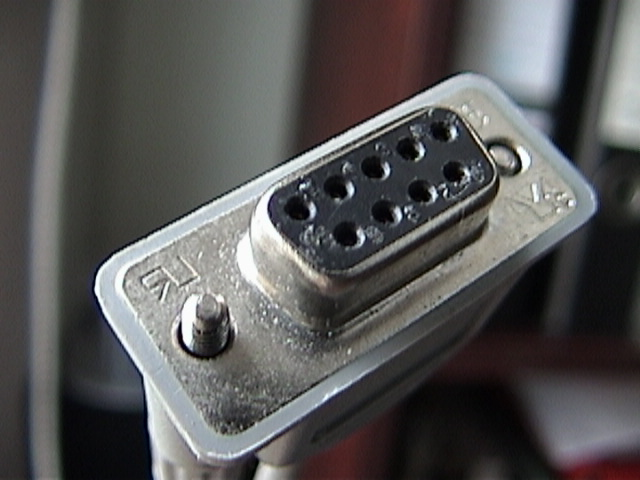
\includegraphics[keepaspectratio,width=0.5\textwidth]{Hardwares/RS-232.jpeg}
	\caption{RS-232 DB-9连接器}
	\label{figRs232Db9}
	\end{center}
\end{figure}


RS-232指定了20个不同的信号连接,由25个D-sub(微型D类)管脚构成的DB-25连接器。很多设备只是用了其中的一小部分管脚,出于节省资金和空间的考虑不少机器采用较小的连接器,特别是9管脚的D-sub或者是DB-9型连接器被广泛使用绝大多数自IBM的AT机之后的PC机和其他许多设备上。DB-25和DB-9型的连接器在大部分设备上是雌型,但不是所有的都是这样。最近,8管脚的RJ-45型连接器变得越来越普遍,尽管它的管脚分配相差很大。EIA/TIA 561标准规定了一种管脚分配的方法,但是由Dave Yost发明的被广泛使用在Unix计算机上的Yost串连设备配线标准("Yost Serial Device Wiring Standard")以及其他很多设备都没有采用上述任一种连线标准。

\subsection{EIA-422和EIA-485}
EIA-422(过去称为RS-422)是一系列的规定采用4线,全双工,差分传输,多点通信的数据传输协议。
EIA-422 的通常用途是作为RS-232的扩展。
EIA-485(过去叫做RS-485 或者RS485)是隶属于OSI模型物理层的电气特性规定为2线,半双工,多点通信的标准。它的电气特性和RS-232大不一样。
EIA-485仅仅规定了接受端和发送端的电气特性。它没有规定或推荐任何数据协议。EIA-485可以应用于配置便宜的广域网和采用单机发送,多机接受通信链接。
EIA-485在使用四线时可以和EIA-422一样实现全双工。

目前EIA-422 (RS-422) 与 EIA-485 (RS-485) 的应用主要集中在工业控制环境,特别是长距离数据传输,如连接远程周边控制器或传感器。

EIA-485 的用途:
\begin{itemize}
\item
    SCSI-2和SCSI-3通常使用这种标准的设备来作为物理层。
\item
    EIA-485 经常和常用设备UART一起使用来实现在飞机上的低速率数据传输,举个例子,一些乘客控制单元采用这种设备,从而只需要很少的线缆就可以实现几个椅子共享线缆,从而减轻整个设备的重量。
\item
    EIA-485 同样可以在一些工厂的项目控制机器上看到,来实现工厂不同楼层之间的数据通信。它可以抵抗机械设备和焊接设备的电磁干扰。
\item
    EIA-485 在大型音频系统中使用,可以在音乐厅和剧院见到这种设备,可以使用普通的计算机来运行一些特殊的软件实现远距离音频设备的控制。EIA-485通过XLR标准的线缆连接的设备大量的用于麦克风上,从而实现舞台和控制台之间的连接而不需要预设线路。
\end{itemize}


\subsection{MII}
以太网接口通常包括MAC(媒体接入控制器,Media Access Controller)和PHY(物理接口收发器,PHYsical Interface or transceiver)。
以太网PHY和MAC对应OSI模型的两个层——物理层和数据链路层。


MII (Media Independent Interface(介质无关接口);或称为媒体独立接口,它是IEEE-802.3定义的以太网行业标准。它包括一个数据接口,以及一个MAC和PHY之间的管理接口。数据接口包括分别用于发送器和接收器的两条独立信道。每条信道都有自己的数据、时钟和控制信号。MII数据接口总共需要16个信号。管理接口是个双信号接口:一个是时钟信号,另一个是数据信号。通过管理接口,上层能监视和控制PHY。MII (Management interface)只有两条信号线。

MII标准接口用于连接Fast Ethernet MAC-block与PHY。"介质无关"表明在不对MAC硬件重新设计或替换的情况下,任何类型的PHY(双绞线,光纤)设备都可以正常工作。在其他速率下工作的与 MII等效的接口有:AUI(10M以太网)、GMII(Gigabit以太网)和XAUI(10-Gigabit以太网)。

\begin{figure}[ht]
	\begin{center}
		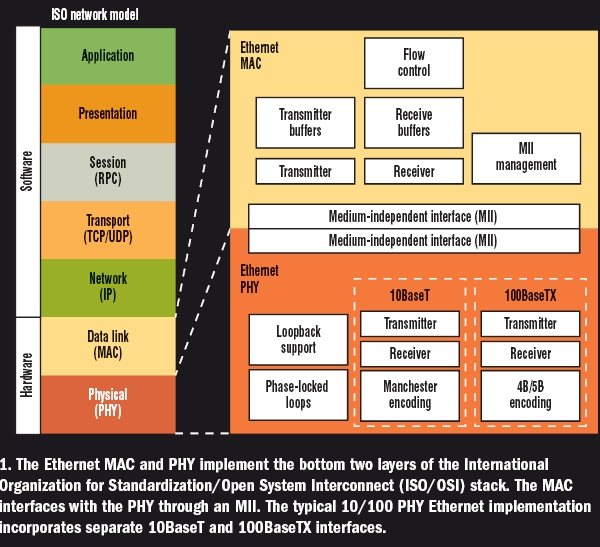
\includegraphics[keepaspectratio,width=0.5\textwidth]{Hardwares/MII.jpg}
	\caption{MII在OSI模型中的位置}
	\label{figOsiMii}
	\end{center}
\end{figure}



MII支持10兆和100兆的操作,一个接口由14根线组成,它的支持还是比较灵活的,但是有一个缺点是因为它一个端口用的信号线太多,如果一个8端口的交换机要用到112根线,16端口就要用到224根线,到32端口的话就要用到448根线,一般按照这个接口做交换机,是不太现实的,所以现代的交换机的制作都会用到其它的一些从MII简化出来的标准,比如RMII、SMII、GMII等。

RMII是简化的MII接口,在数据的收发上它比MII接口少了一倍的信号线,所以它一般要求是50兆的总线时钟。RMII一般用在多端口的交换机,它不是每个端口安排收、发两个时钟,而是所有的数据端口公用一个时钟用于所有端口的收发,这里就节省了不少的端口数目。RMII的一个端口要求7个数据线,比MII少了一倍,所以交换机能够接入多一倍数据的端口。和MII一样,RMII支持10兆和100兆(Mbit/s)的总线接口速度。

SMII是由思科提出的一种媒体接口,它有比RMII更少的信号线数目,S表示串行的意思。因为它只用一根信号线传送发送数据,一根信号线传输接受数据,所以在时钟上为了满足100的需求,它的时钟频率很高,达到了125兆,为什么用125兆,是因为数据线里面会传送一些控制信息。SMII一个端口仅用4根信号线完成100信号的传输,比起RMII差不多又少了一倍的信号线。SMII在工业界的支持力度是很高的。同理,所有端口的数据收发都公用同一个外部的125M时钟。

GMII是千兆网(1000 Mbit/s)的MII接口,这个也有相应的RGMII(Reduced Media Independent Interface)接口,表示简化了的GMII接口, 引脚减少了一半。

TMII是200兆速率的MII接口,MII接口为25MHz频率,TMII接口为50MHz频率。

SGMII(Serial Gigabit Media Independent Interface)是PHY与MAC之间的接口,类似与GMII和RGMII,只不过GMII和RGMII都是并行的,而且需要随路时钟,PCB布线相对麻烦,而且不适应背板应用。而SGMII是串行的,不需要提供另外的时钟。SGMII用于千兆网,也支持10/100 MBit Ethernet。


XGMII(10 Gigabit Media Independent Interface,X是罗马数字) 能达到10Gb速率。

XAUI(10 Ethernet Attachment Unit Interface)是XGMII的延伸,XAUI位于MAC末端的XGXS、和PHY末端的XGXS之间。XAUI延伸了XGMII的操作长度并减少了信号接口的数目。应用范围包括延伸MAC和PHY模组之间的实体分隔以10.0 Gbit/s 以太系统分散横跨电路板。




























